\documentclass{article}

\usepackage[final]{corl_2026}
\usepackage{graphicx}
\usepackage{booktabs}
\usepackage{amsmath}
\usepackage{array}
\usepackage{url}
\setlength{\textfloatsep}{6pt}
\setlength{\floatsep}{6pt}
\setlength{\intextsep}{6pt}

\title{Reward Shaping and Curriculum PPO for Sparse-Reward SoccerTwos Control}

\author{
  Vedaang Chopra\\
  Georgia Institute of Technology\\
  United States\\
  \texttt{vedaangchopra@gatech.edu}
}

\begin{document}
\maketitle


\begin{abstract}
This project studies PPO training in SoccerTwos, a sparse-reward Unity soccer environment where the agent has to learn ball-contact and goal-scoring behavior from limited feedback. We started with a plain PPO baseline, then tested two changes: reward shaping with small progress bonuses, and curriculum learning with easier start states early in training. The baseline struggled with exploration and reached 0.2399 mean episode reward after 2.0M environment steps. Reward shaping improved the same-budget result to 0.4036, but the first curriculum run did much better, reaching 1.7869 after 2.06M steps. We then resumed the best curriculum checkpoint for a longer v3 run. The final \texttt{TEAMNAME\_v3\_AGENT} reached 1.9692 final mean episode reward after about 30M steps and won 8 of 10 recorded matches against the PPO baseline. Overall, the curriculum run was the clearest improvement, mainly because it made early exploration less random and gave the agent easier chances to learn useful ball behavior.
\end{abstract}

\keywords{Reinforcement Learning, SoccerTwos, Curriculum Learning}


\section{Overview}

SoccerTwos is a two-team Unity soccer environment where cube agents have to move around the field, reach the ball, defend, and score goals. In our experiments, the hardest part was getting useful behavior started. With the default sparse reward, the baseline agent could spend many episodes moving around without getting much feedback, so learning was slow early on.

We used PPO as the base method because it was already supported in the RLlib project setup and was stable enough for the Unity rollouts. From that baseline, We tried two changes. First, We added reward shaping so the agent received small rewards for moving toward the ball and moving the ball toward the opponent goal. Second, We used curriculum learning, where the agent started from easier game states before moving to harder ones. The final submitted policy, \texttt{TEAMNAME\_v3\_AGENT}, came from resuming the best curriculum checkpoint and training it for a longer budget.


% \begin{figure}[t]
%     \centering
%     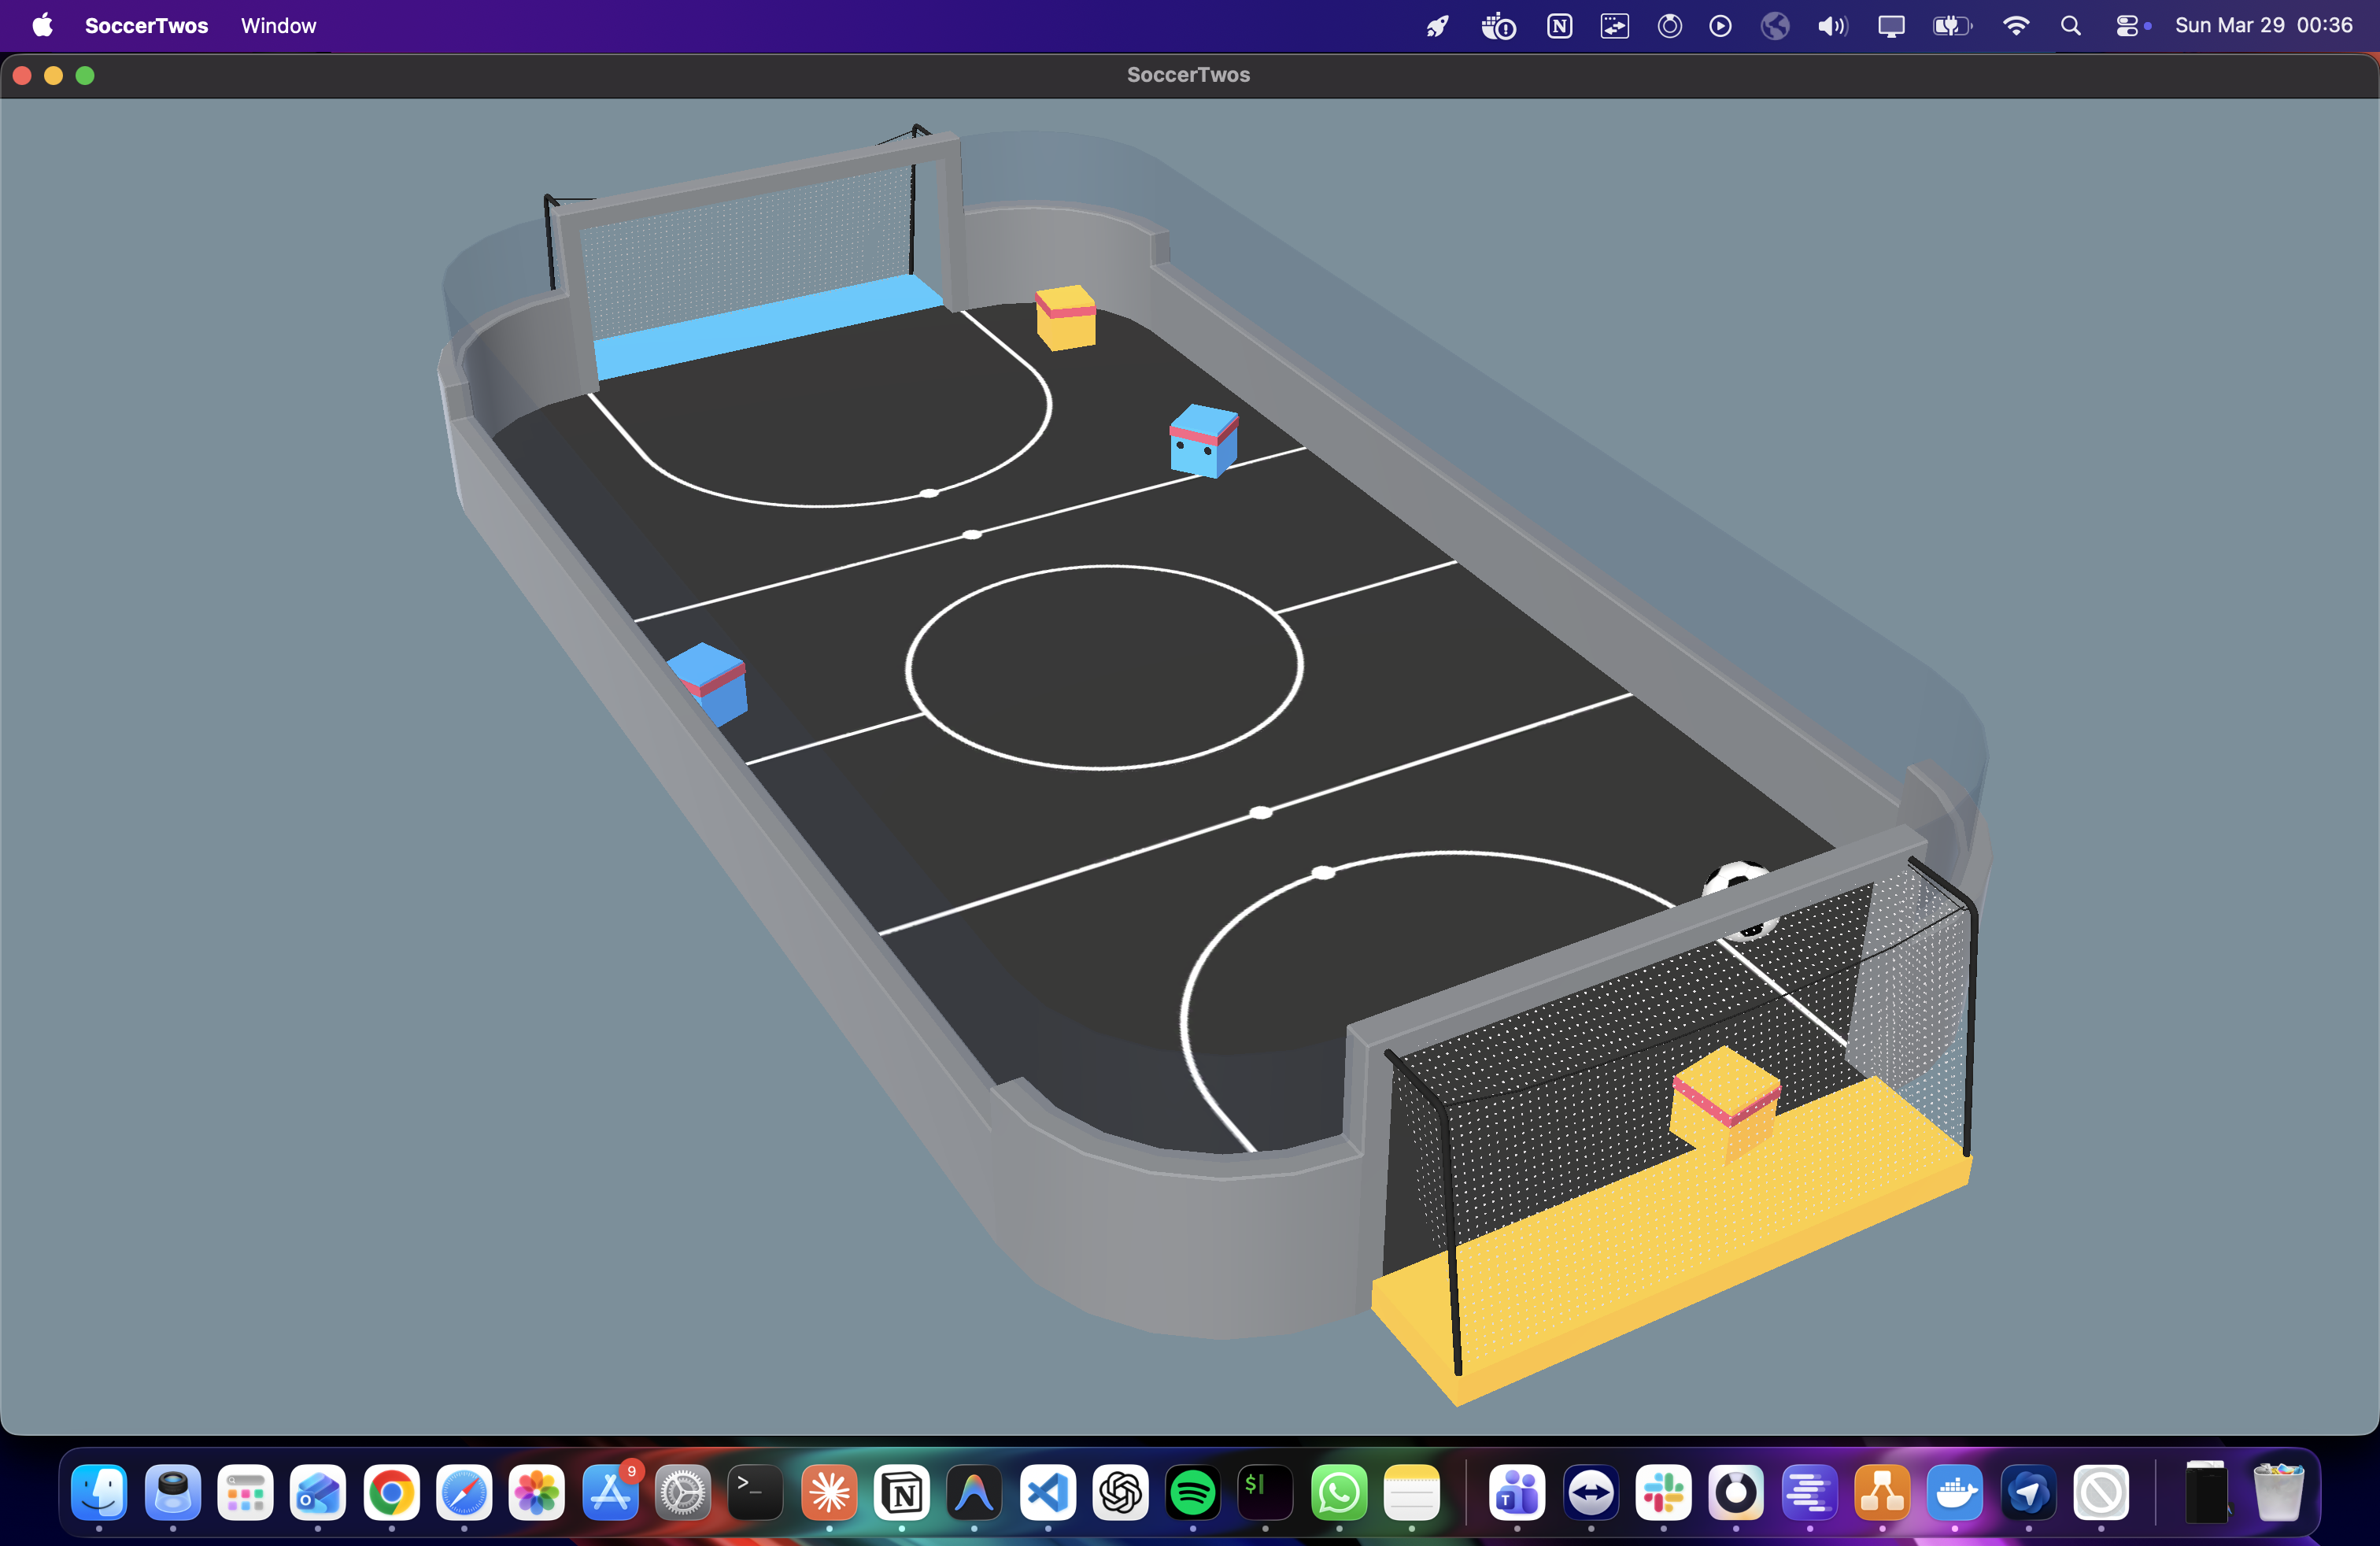
\includegraphics[width=0.65\linewidth]{figures/envt.png}
%     \caption{SoccerTwos environment used for training and evaluation. The task requires cube agents to move in the arena, interact with the ball, and score in the opponent goal.}
%     \label{fig:env_screenshot}
% \end{figure}



\section{Method Description}

\textbf{PPO baseline.}
We used Proximal Policy Optimization (PPO) as the baseline because it was already supported in the RLlib training setup. The baseline used the default sparse SoccerTwos reward and a feed-forward ReLU actor-critic network. For the baseline and reward-shaped runs, the policy and value model used one hidden layer of width 512 with shared value layers.

\textbf{Reward-shaped PPO.}
The first change We tried was dense reward shaping during training. The idea was to give the agent some feedback before it actually scored or conceded. We used the environment \texttt{info} dictionary to compute the player-to-ball distance \(d_{pb}\) and the ball-to-goal distance \(d_{bg}\). At each transition, the wrapper added
\[
r_{\mathrm{shape}} =
\mathrm{clip}\left(0.01(d_{pb}^{t-1}-d_{pb}^{t}) +
0.02(d_{bg}^{t-1}-d_{bg}^{t}), -0.05, 0.05\right).
\]
This gives a small positive reward when the player gets closer to the ball or when the ball moves closer to the opponent goal. We clipped the bonus to \(\pm 0.05\) so it would guide exploration without becoming the main objective. This shaping was only used during training, so the exported policy does not need the privileged \texttt{info} fields at inference time. The motivation is the usual sparse-reward reward-shaping idea~\citep{ng1999policy}.

\textbf{Curriculum PPO.}
The second change was curriculum learning. Instead of always starting from the full game setup, We started the agent from easier states and then increased the difficulty. A callback set the initial ball and player states through the Unity environment channel. The curriculum used five stages, going from ``Very Easy Goal'' to ``Random Players,'' and advanced when the running \texttt{episode\_reward\_mean} passed 1.5. This made early training less random because the agent had more reachable chances to learn ball-to-goal behavior.

The curriculum policy also used a two-layer ReLU MLP with hidden layers \([256,256]\) and shared value layers. This means the curriculum comparison is not a perfectly isolated ablation, since both the start-state distribution and the network changed. Still, curriculum was the main intended change because it directly targeted the exploration issue we saw in the baseline. The final v3 policy resumed the strongest curriculum checkpoint and extended training to about 30.0M environment steps~\citep{bengio2009curriculum}.

\textbf{Final hyperparameters.}
The submitted policy was trained with Ray RLlib PPO using the PyTorch backend. The final v3 run used learning rate \(5\times10^{-5}\), discount factor \(\gamma=0.99\), PPO clipping parameter 0.3, 30 SGD epochs per update, train batch size 80{,}000, minibatch size 8{,}000, rollout fragment length 2{,}000, gradient clipping at 0.5, 40 rollout workers, and 1 GPU. The exported submission package was \texttt{TEAMNAME\_v3\_AGENT}.

\begin{table}[t]
\centering
\small
\caption{Main PPO training configurations used in the project.}
\label{tab:methods}
\begin{tabular}{lccc}
\toprule
Method & Reward & Curriculum & Network \\
\midrule
PPO baseline & sparse & no & [512] \\
Reward-shaped PPO & sparse + shaping & no & [512] \\
Curriculum PPO & sparse + curriculum setup & yes & [256, 256] \\
Curriculum PPO v3 & resumed curriculum & yes & [256, 256] \\
\bottomrule
\end{tabular}
\end{table}



% --------------------------------------------------------------------------------


\section{Results and Evaluation}

Figure~\ref{fig:curves} compares the main training runs. The sparse-reward PPO baseline reached 0.2399 mean episode reward after 2.0M environment steps. Reward-shaped PPO improved this to 0.4036 at the same budget, so the shaping signal helped, but not enough to solve the task. The first curriculum run was the clear jump, reaching 1.7869 mean reward after 2.06M steps. We then resumed the best curriculum checkpoint for the longer v3 run, which reached 1.9692 final mean reward, with a best logged mean reward of 1.9705 at 29.85M steps.

The v3 result is not a perfectly fair same-budget comparison against the baseline, since it used a much longer training budget. We include it because it was the final submitted policy. For judging the method change itself, the cleaner comparison is the 2M-step baseline, reward-shaped PPO, and first curriculum PPO runs. In that comparison, curriculum learning was the strongest result.

\begin{figure}[t]
\centering
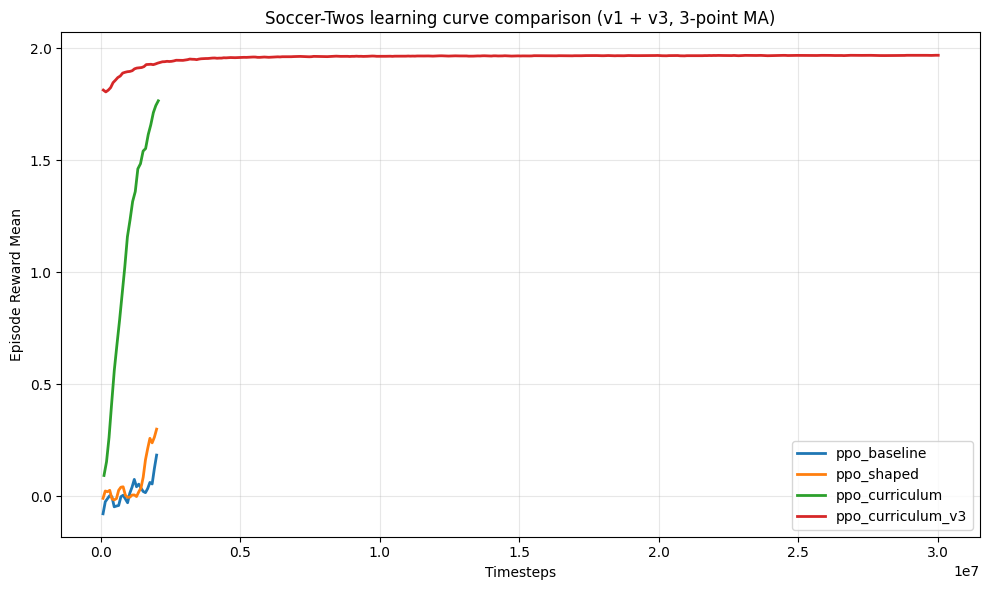
\includegraphics[width=0.92\linewidth]{figures/all_comaprison.png}
\caption{Training reward curves. The first three runs give the closest same-budget comparison; v3 is the longer final submission run.}
\label{fig:curves}
\end{figure}

Table~\ref{tab:eval} shows the recorded headless evaluation matches for the final curriculum v3 policy. The number of episodes is small, so We treat these results as supporting evidence rather than a final statistical conclusion. The v3 policy won 8 of 10 matches against the PPO baseline and 6 of 10 matches against the earlier curriculum policy. This lines up with the training curves: v3 was clearly better than the baseline and somewhat better than the earlier curriculum checkpoint.

\begin{table}[t]
\centering
\small
\caption{Recorded headless evaluation summaries for the final curriculum v3 policy.}
\label{tab:eval}
\begin{tabular}{lrrrr}
\toprule
Matchup & Episodes & Wins & Agent mean & Opponent mean \\
\midrule
Curriculum v3 vs. baseline & 10 & 8 & 1.1140 & -1.2084 \\
Curriculum v3 vs. curriculum & 10 & 6 & 0.3407 & -0.4258 \\
\bottomrule
\end{tabular}
\end{table}

\begin{figure}[t]
\centering
\begin{minipage}[t]{0.48\linewidth}
  \centering
  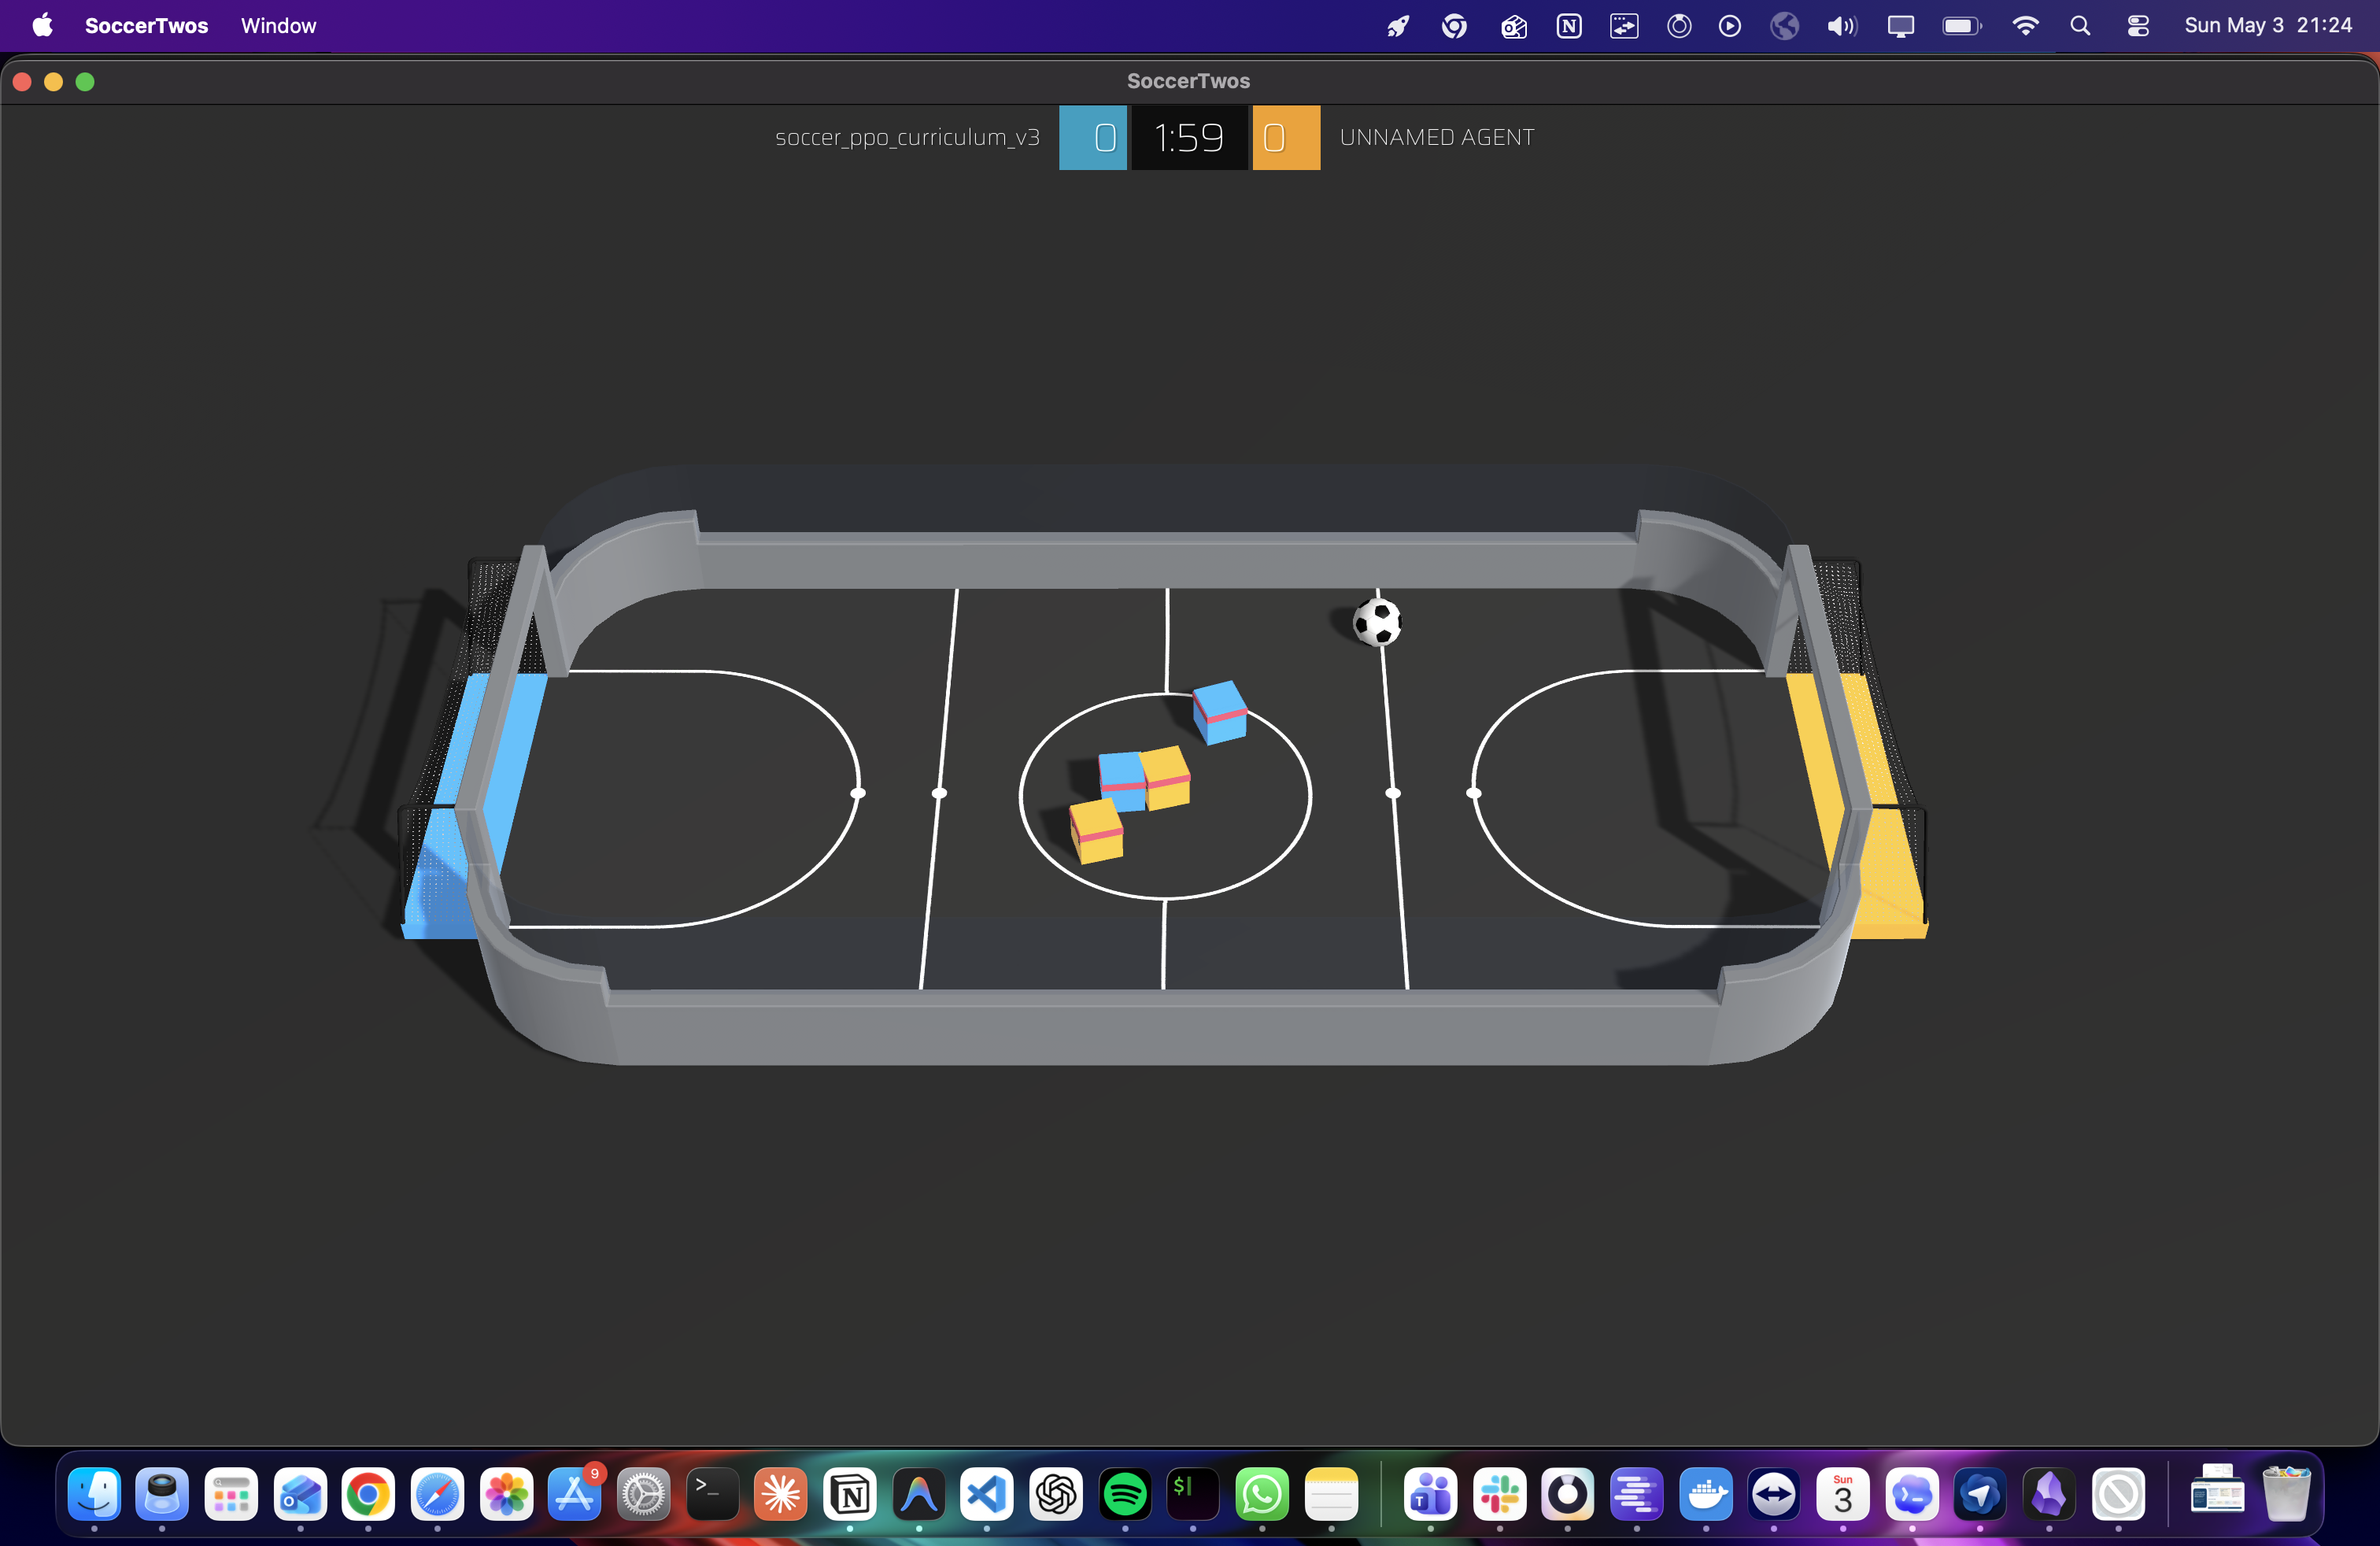
\includegraphics[width=\linewidth]{figures/figure-gameplay-1.png}
\end{minipage}
\hfill
\begin{minipage}[t]{0.48\linewidth}
  \centering
  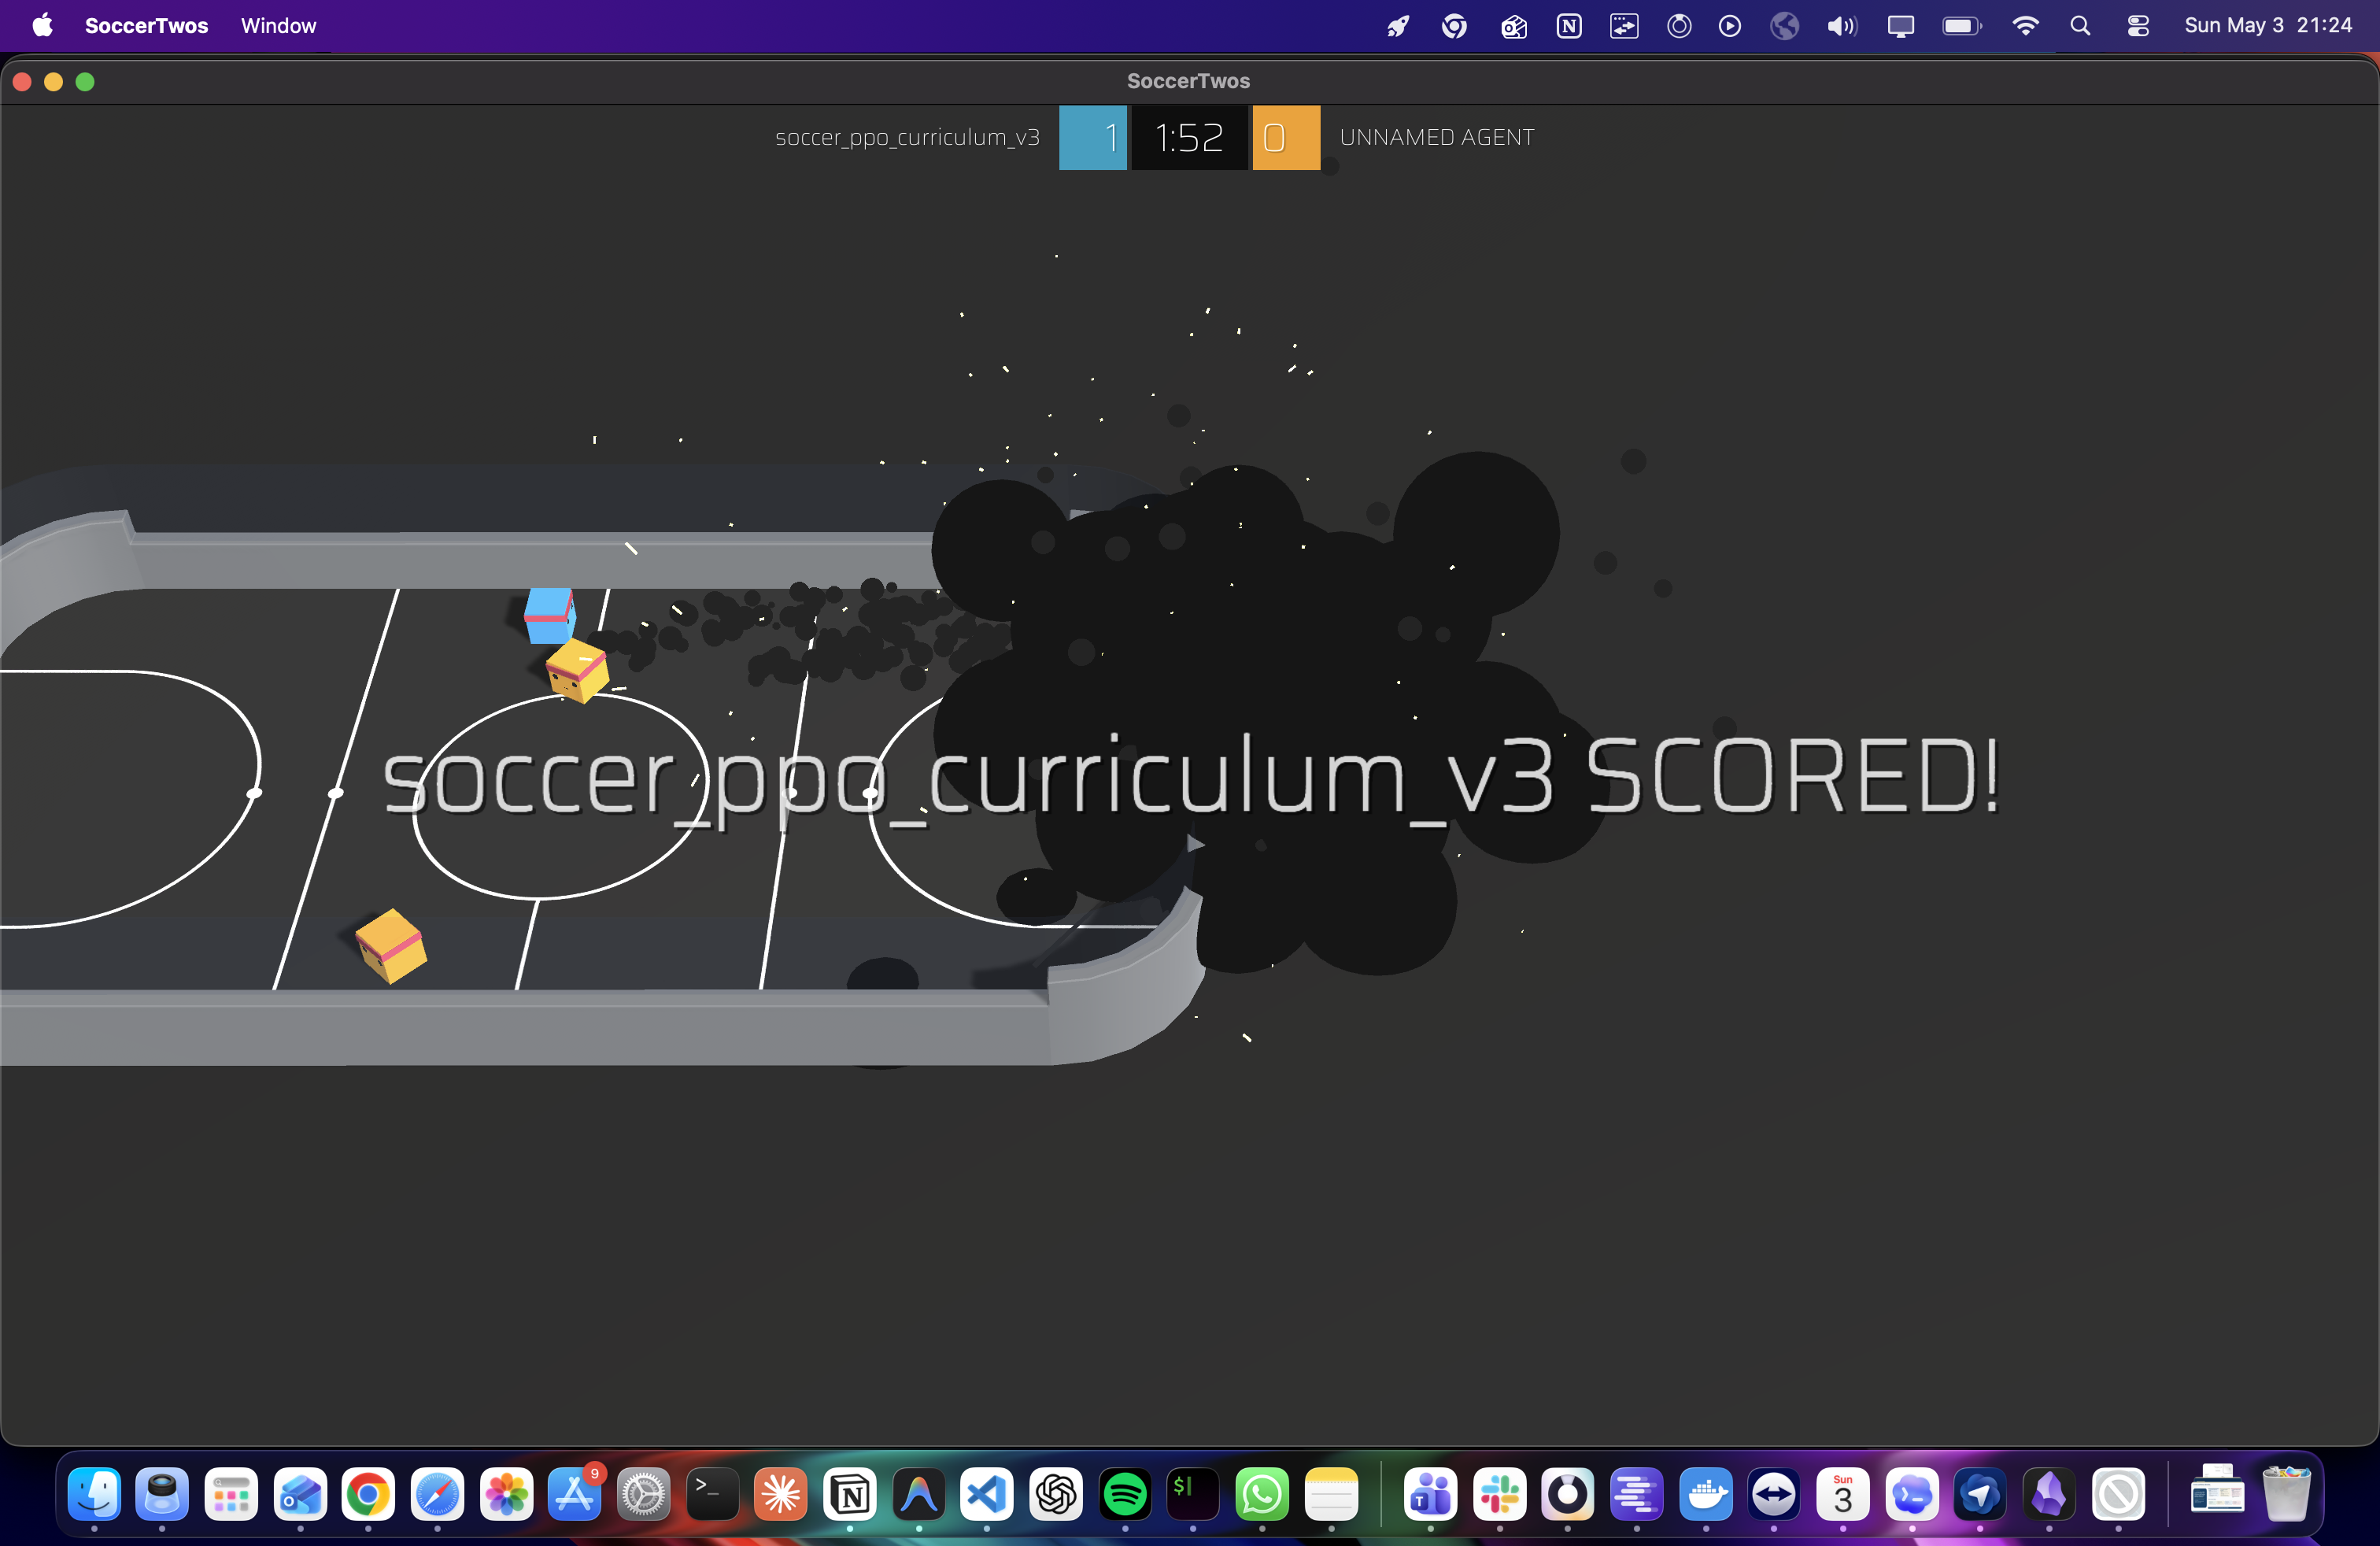
\includegraphics[width=\linewidth]{figures/fig-gameplay-2.png}
\end{minipage}
\caption{Representative evaluation frames for the final curriculum v3 policy.}
\label{fig:gameplay}
\end{figure}

Figure~\ref{fig:v3_diagnostics} shows the detailed diagnostics for the final curriculum v3 run. The mean episode reward approached 2.0 and stayed stable near the end of training. Episode length also dropped and then stabilized, which suggests the policy was reaching terminal soccer outcomes faster. The entropy and value-loss curves also looked reasonable near the end of training.

\begin{figure}[t]
\centering
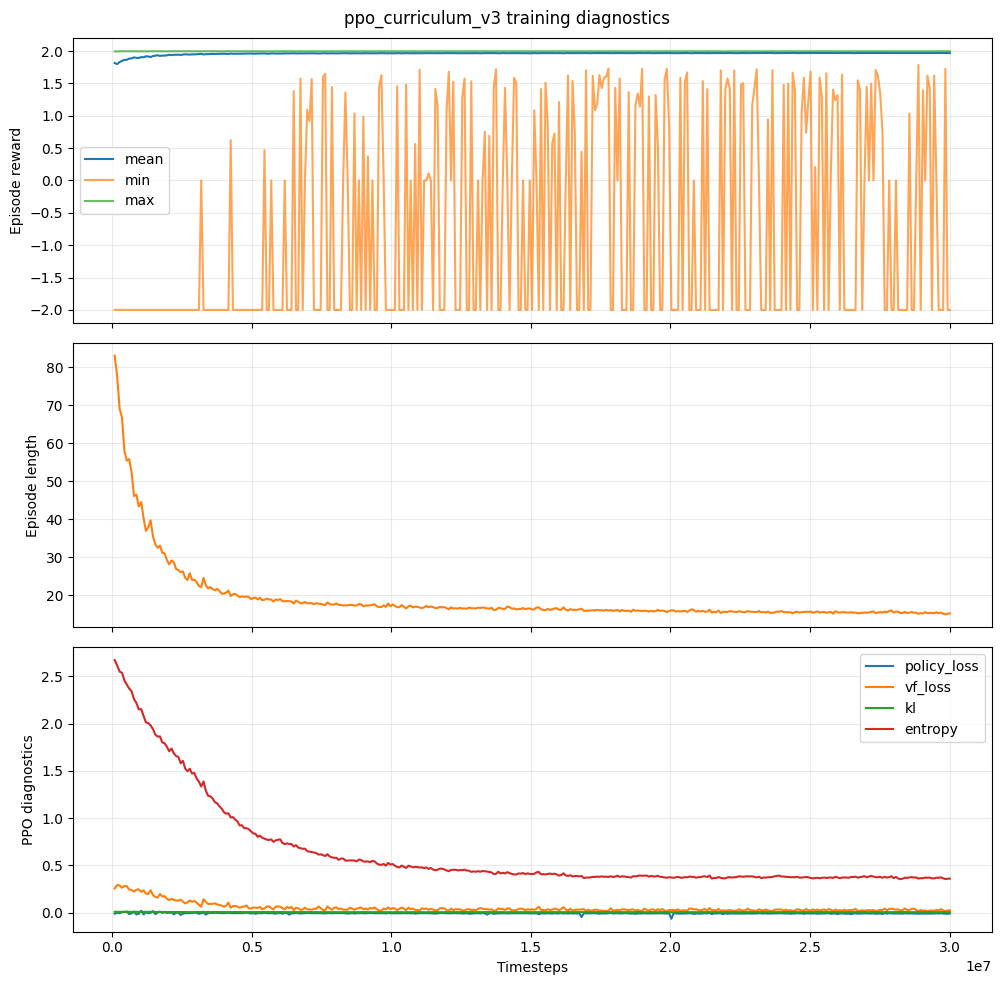
\includegraphics[width=0.92\linewidth]{figures/best_rl_algo.png}
\caption{Final curriculum v3 training diagnostics.}
\label{fig:v3_diagnostics}
\end{figure}

% --------------------------------------------------------------------------------


\section{Reward, Observation, and Architecture Modifications}

\textbf{Reward.}
The reward-level change was the training-only \texttt{RewardShapingWrapper}. It used \texttt{player\_info} and \texttt{ball\_info} to reward two kinds of progress: the player moving closer to the ball, and the ball moving closer to the opponent goal. The shaping bonus was clipped to \(\pm 0.05\), so it stayed small compared with scoring rewards. This helped early learning, but reward shaping alone did not match the curriculum runs.

\textbf{Observation and action handling.}
We did not add a custom observation wrapper or change the Unity-side observations. The final policy uses the provided 336-dimensional SoccerTwos observation vector. The main interface issue was action formatting: training used flattened \texttt{Discrete(27)} actions, while live matches used branched \texttt{MultiDiscrete([3,3,3])} actions. Since We did not add custom observation features, We do not count observation design as one of my modifications.

\textbf{Architecture and curriculum.}
The baseline and reward-shaped PPO agents used one hidden layer of width 512. The curriculum agents used a two-layer \([256,256]\) ReLU MLP with shared value layers. The curriculum also changed the start-state distribution by beginning with easier near-goal states and gradually moving to harder ball and player placements. Since architecture and curriculum changed together, this is not a perfectly isolated ablation. Still, the curriculum directly addressed the baseline's main failure mode: long early training with little useful reward feedback.

\section{Limitations and Future Work}

The main limitation is evaluation size. My strongest recorded comparison against the PPO baseline used 10 headless episodes, not a larger 100-episode evaluation, so the match results should be treated as preliminary. The training setup was also simplified because the agent trained in a single-player setting against a fixed opponent policy. Because of that, the final policy should not be treated as learning full multi-agent soccer behavior such as passing, coordinated defense, or team positioning.

Another limitation is attribution. The curriculum runs changed both the start-state distribution and the network architecture, so We cannot fully separate which part caused the improvement. Based on the baseline behavior, We think the curriculum was the bigger factor, but a cleaner ablation would keep the architecture fixed and only change the curriculum.

We also explored imitation learning, but it was not part of the final successful method. Future work should run larger evaluations against random, baseline, and TA agents; compare reward-shaped PPO directly against curriculum v3 in head-to-head matches; and test whether the curriculum policy stays robust under self-play or stronger multi-agent opponents.


\section{GitHub Link}
\url{https://github.com/Vedaang-Chopra/RL_Soccer_project}

\section*{Acknowledgments}

We used ChatGPT~\citep{openai2026chatgpt} and Gemini~\citep{google2026gemini} for writing feedback, editing suggestions, code editing, bug fixing, and \LaTeX{} cleanup. All experiments, implementation choices, reported results, and final claims were reviewed and verified by the authors.

\bibliography{example}

\end{document}
